%!TeX root=../tese.tex
%("dica" para o editor de texto: este arquivo é parte de um documento maior)
% para saber mais: https://tex.stackexchange.com/q/78101/183146

%% ------------------------------------------------------------------------- %%
\chapter{Introdução}
\label{cap:introducao}

Árvores Binárias de Busca (ABBs) são estruturas de dados que armazenam um conjunto de chaves de um universo estático, que possui uma ordem total, e dão suporte a buscas neste conjunto. Denotaremos por $n$ o número de elementos do conjunto armazenado na ABB considerada.

Estas estruturas são fundamentais na ciência da computação e possuem as mais diversas finalidades. Nesse projeto iremos estudar a chamada Conjectura da Otimalidade Dinâmica, interpretações geométricas de algoritmos de busca em ABBs e suas delimitações associadas. Também serão estudadas as árvores splay e as árvores tango.

Adaptando a definição dada por \cite{Sedgewick}, \textit{árvore binária de busca} é uma árvore binária onde cada nó possui uma chave comparável e possivelmente um valor associado. Além disso, os nós satisfazem a restrição de que a chave em qualquer nó é maior do que as chaves em todos os nós na subárvore esquerda desse nó e menor do que as chaves em todos os nós na subárvore direita desse nó.

As ABBs também possuem um atributo \textit{raiz} que aponta para o nó raiz ou possui valor \textit{nulo}, caso a árvore esteja vazia.

\textit{Rotações} são operações que trocam dois nós, pai-filho, entre si enquanto mantém a restrição vista acima. Veja a figura 1. Essa operação é fundamental para garantir performance em alguns algoritmos de ABBs e é muito utilizada para controlar a altura das árvores.


% Arrumar figura!!
\begin{figure}[htbp]
    \centering
    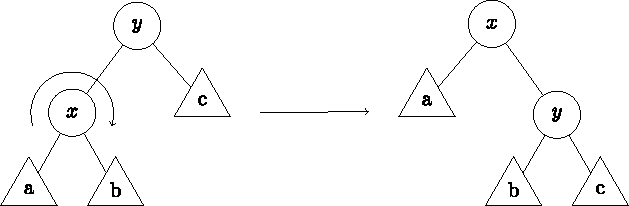
\includegraphics{imagens/zig.pdf}
    \label{fig:imagem}
\end{figure}

No contexto da Conjectura da Otimalidade Dinâmica, apenas serão consideradas buscas bem sucedidas, que chamaremos de \textit{acessos}, e não são consideradas inserções ou remoções no conjunto armazenado. No modelo de computação adotado, um algoritmo de busca em uma ABB, para fazer o acesso a uma chave, mantém um único ponteiro. Chamamos de \textit{nó corrente} o nó apontado por esse ponteiro. 

No início da execução do acesso, o ponteiro aponta para a raiz da árvore e, após uma sequência de operações, deve encontrar o nó que armazena a chave procurada. As operações chamadas de \textit{primitivas} são:
\begin{enumerate}
    \item Mover o ponteiro para o filho esquerdo do nó corrente.
    \item Mover o ponteiro para o filho direito do nó corrente.
    \item Mover o ponteiro para o pai do nó corrente.
    \item Fazer uma rotação que troca a posição do nó corrente e do seu pai.
\end{enumerate}

O algoritmo tradicional de busca em ABB não executa a operação primitiva 4. No modelo de computação adotado, todas essas operações possuem custo unitário. O custo para executar um acesso nesse modelo é o número de operações primitivas executadas até encontrar a chave procurada.

O algoritmo tradicional de busca inicia a execução de um acesso na raiz e desce para o filho apropriado até alcançar a chave procurada. O pior caso é quando a chave procurada está em um nó folha mais profundo. Nesse caso o algoritmo tem que passar por toda a altura da árvore até chegar a essa folha. Assim o custo do pior caso é proporcional a altura da árvore, que pode ser em princípio linear em $n$. 

Com intuito de mitigar o custo do pior caso, algumas ABBs estrategicamente utilizam da operação primitiva 4 (rotação) para balancear o tamanho das subárvores e assim diminuir a altura da árvore. Um exemplo famoso, que daremos mais detalhes a frente, é a árvore splay. Essa ABB executa rotações baseando-se na heurística ``move to front" e assim balanceia a árvore durante as buscas. Essa árvore não utiliza armazenamento adicional para isso.

Como o conjunto armazenado nas ABBs que consideraremos não sofre alterações, podemos assumir que esse conjunto é \{1,2,\ldots,$n$\}.

ABBs \textit{online} são ABBs que apenas possuem informações sobre os acessos passados. Ou seja, ao acessar $x_{i}$, o algoritmo de busca não tem conhecimento das chaves $x_{i+1},\ldots,x_{m}$, nem mesmo do valor de $m$. Em particular, muitas ABBs online possuem informações adicionais em cada nó que auxiliam o algoritmo de busca a decidir quando executar rotações durante a busca pelas chaves procuradas. Qualquer ABB online que usa O$(1)$ palavras adicionais por nó possui tempo de execução dominado pelo número de operações primitivas.

Uma ABB é chamada de \textit{offline} se tem conhecimento de $X$ antes de começar os acessos as chaves de $X$. Nesse contexto, o comportamento do algoritmo não depende unicamente do histórico de acessos passados, uma vez que possui conhecimento prévio de toda a sequência de chaves a serem acessadas.

Dada uma sequência $X$ de \textit{acessos}, uma ABB é considerada ótima se executa os acessos por $X$ com o menor custo possível. Podemos definir OPT$(X)$ como o número de operações primitivas realizadas pela ABB ótima para a sequência $X$. Em outras palavras, OPT$(X)$ é o menor número de operações primitivas necessárias para uma ABB concluir todos os acessos de $X$. 

ABBs balanceadas estabelecem que OPT$(X)$ = O$(m \lg n)$, onde $n$ é o número de chaves armazenadas na árvore e $m$ é o comprimento de $X$. Como já observado, $\text{OPT}(X) \geq m$. Wilber \cite{lowerbound_wilbert} provou que OPT$(X)$ = $\Theta$$(m \lg n)$ para algumas classes de sequências $X$. 

Uma ABB online é \textit{dinamicamente ótima} se, para todas as sequências $X$, seu algoritmo de busca tem custo O(OPT($X$)). De maneira mais geral, uma ABB online é $c$-competitiva se executa todas as sequências $X$ suficientemente longas com custo no máximo $c$\,OPT($X$).

Todo esse estudo foi feito para tentar responder à pergunta: ``\textit{Existe uma ABB online dinamicamente ótima?}".

Uma das tentativas de responder tal pergunta foi a árvore splay de Sleator e Tarjan~\cite{selfadjustingbst}. Árvores splay são ABBs que seguem a heurística ``move to front". Assim, após cada acesso, a árvore se reestrutura de uma maneira particular, trazendo o nó da chave que foi acessada para a raiz da árvore.

Apesar de existirem muitas ABBs muito bem documentadas com tempo por busca logarítmico em $n$, essas estruturas normalmente não conseguem alcançar uma eficiência superior a isso independentemente da entrada. Padrões de acesso do mundo real muitas vezes possuem estruturas repetitivas, como por exemplo bancos de dados que recebem solicitações frequentes para um pequeno número de elementos de alto tráfego. Em alguns desses casos, é possível ter uma performance melhor que O$(\lg n)$ por acesso utilizando árvore splay, uma vez que essa eventualmente ficaria com as chaves mais acessadas mais próximas à raiz da árvore. 

Há uma conjectura não resolvida no artigo \cite{selfadjustingbst} que diz que as árvores splay são dinamicamente ótimas. Essa conjectura ficou conhecida como a Conjectura da Otimalidade Dinâmica.

A árvore conhecida que mais se aproxima de uma árvore ótima é a árvores tango~\cite{dynamicoptimality}. Tal estrutura é O$(\lg \lg n)$-competitiva. Esta árvore utiliza de O$(\lg \lg n)$ bits a mais por nó e o custo para determinar a próxima operação primitiva a ser executada é amortizadamente constante.

Nas árvores tango, há a definição de \textit{filho preferido}. O \textit{filho preferido} de um nó é o filho direito se ele foi o nó mais recentemente acessado em comparação com o nó esquerdo, e caso contrário (incluindo o caso em que nenhum dos dois filhos foi acessado ainda), definimos o nó esquerdo como \textit{filho preferido}.

Define-se então um \textit{caminho preferido} como um caminho maximal de um nó da ABB até a folha que passa apenas por \textit{filhos preferidos}. 

Os caminhos preferidos particionam os nós da árvore. Nas árvores tango, os nós de cada caminho preferido são armazenados em uma ABB balanceada tendo como chave a profundidade do nó no caminho. Essas árvores auxiliares estão interligadas de uma maneira apropriada.

Durante os \textit{acessos}, os \textit{filhos preferidos} podem ser alterados e isso provocará mudanças nas estruturas da árvores auxiliares para manter a estrutura da árvore tango coerentes com o comportamento descrito acima.
